\chapter{Vecchio vs. Nuovo}
La storia dei videogiochi inizia qualche anno dopo la fine della seconda guerra mondiale, anche se si sono ottenuti risultati concreti solo agli inizi degli anni 70. Nessuno si sarebbe mai aspettato,  nel giro di soli 50 anni da allora, un drastico cambiamento nel concetto stesso che sta alla base del termine "videogioco".
\section{Alba dei videogiochi}
È nel 1972 che nasce la prima effettiva console di gioco destinata al pubblico. Per la prima volta nella storia dell’umanità, l’utente è potuto diventato il protagonista di ciò che accadeva sul televisore senza limitarsi a guardarlo e basta. Il Magnavox Odyssey (così era chiamata la console) era stato concepito per giocare ad un prototipo di videogioco basato sul tennis. Nello stesso anno dell’uscita dell’ Odyssey nacque Atari, l’azienda che portò un’enorme rivoluzione videoludica che diede origine ad un nuovo mercato, quello dei videogiochi. Grazie al celebre \textit{PONG}, gioco progettato sotto la stessa luce del suo unico predecessore, Atari vendette oltre 19.000 cabinati. Si può dire che \textit{PONG} è stato il vero cavallo di battaglia che ha dato inizio a quello che viene definita età dell’oro dei videogames. Durante questo periodo nacquero grandissimi successi a livello mondiale, come Space Invaders e Pac-Man.\\I primi videogiochi per console casalinghe erano in realtà principalmente porting della versione giá uscita sui cabinati per sale giochi. Ai tempi il porting era molto famoso, si può evincere dal fatto che alcuni giochi di quegli anni avessero l’apposita funzione per l’aggiunta di crediti tramite un tasto al posto dei gettoni. Molti videogiochi però subivano anche cambiamenti radicali, al punto di sembrare completamente differenti dalla versione originale. Un esempio schiacciante si può notare nelle due versioni di Outrun, rispettivamente per Arcade e per SEGA Master System (Figura~\ref{fig:outrun}).\\
\begin{figure}[h!]
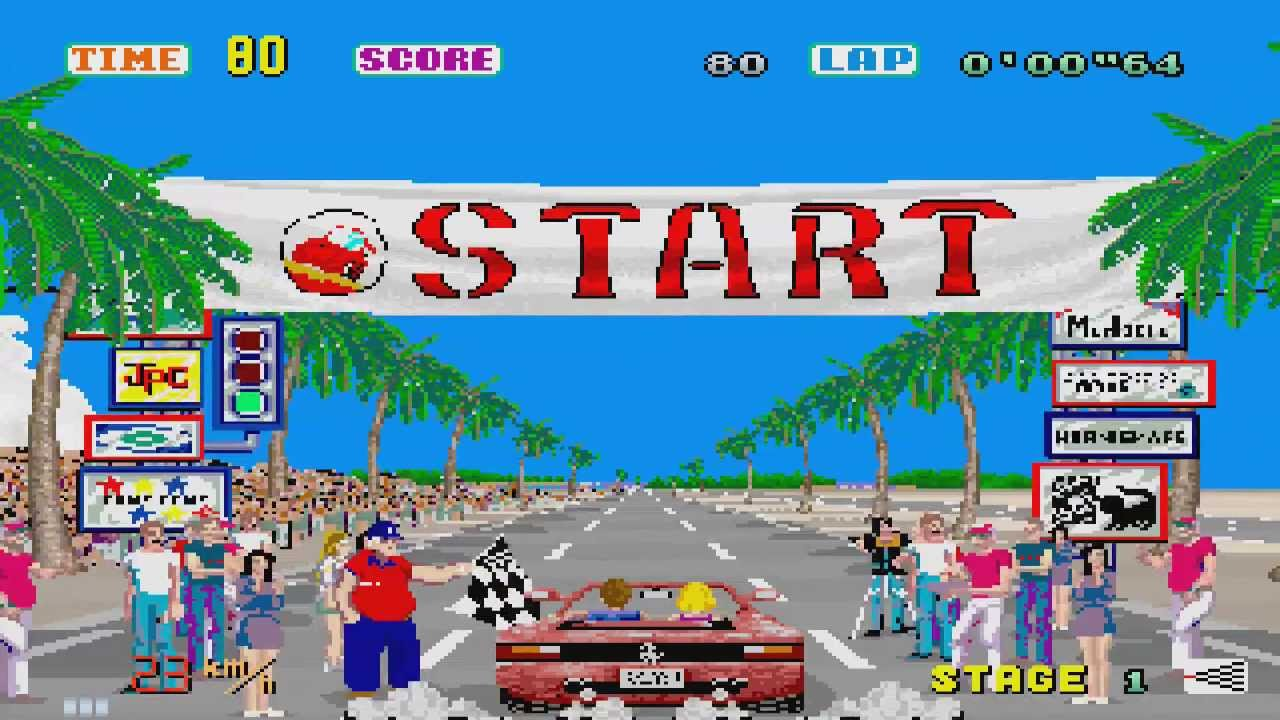
\includegraphics[width=6cm, height=4cm]{outrunarcade}
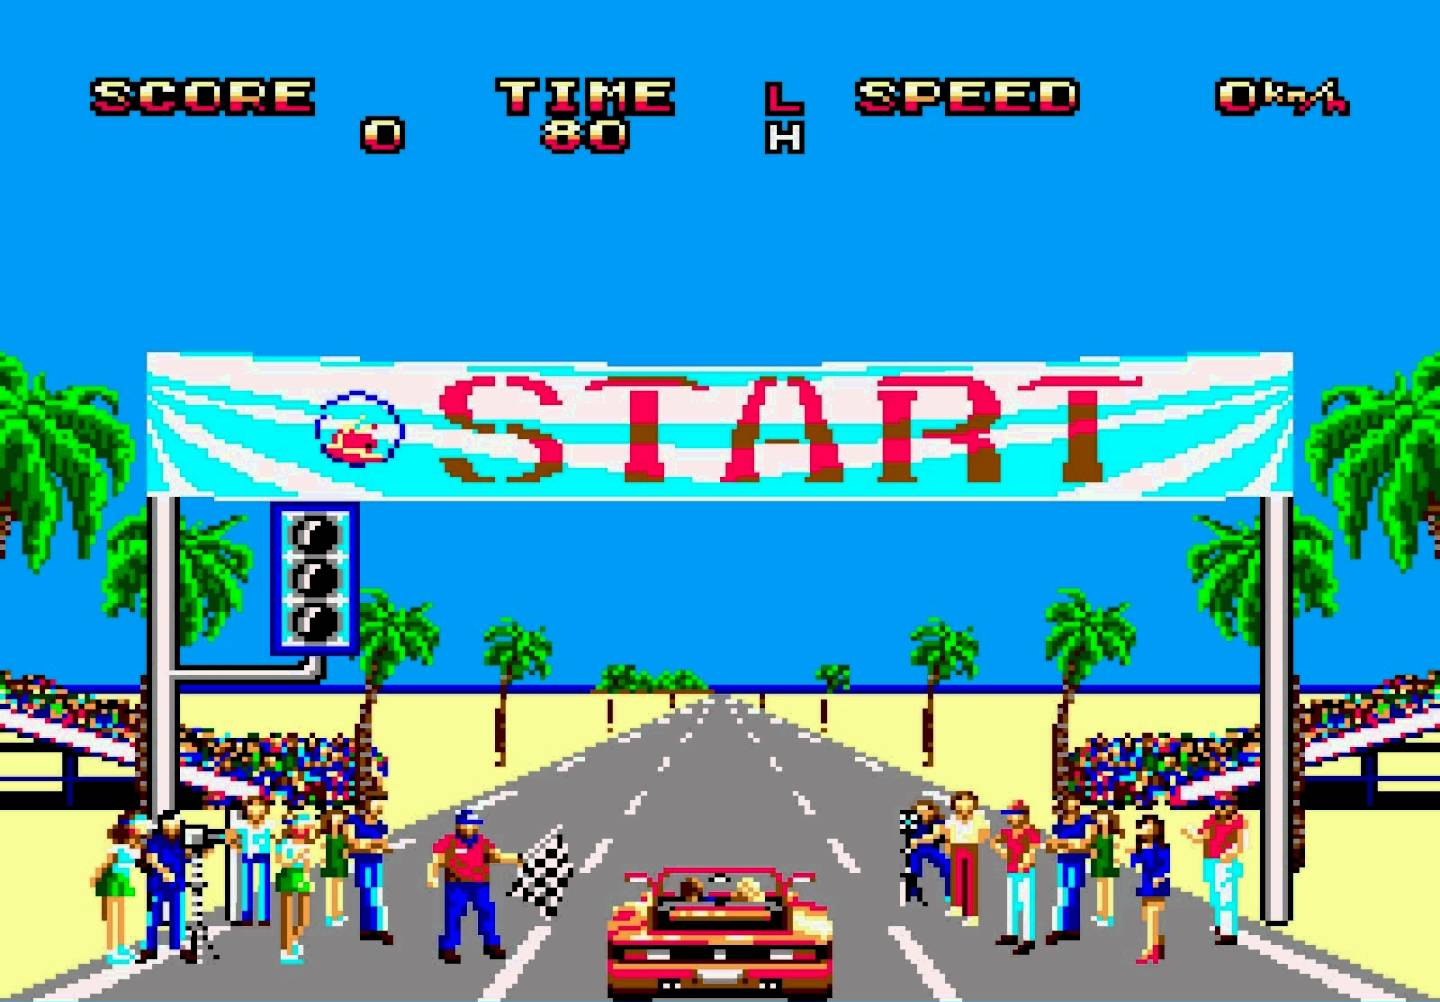
\includegraphics[width=6cm, height=4cm]{outrunmaster}
\caption{Confronto tra le due versioni di Outrun}
\label{fig:outrun}
\end{figure}
\\Il picco della popolarità si toccò negli anni novanta, quando anche la famosa azienda giapponese Sony inventò la sua prima Console: PlayStation.\\La PlayStation aveva una particolarità: era in grado di leggere i giochi dai CD-ROM. La scelta di Sony di puntare tutto sui CD funzionò nel migliore dei modi. La console era in grado anche di leggere CD musicali e diventare un vero e proprio Stereo. Inoltre, essendo una tecnologia molto poco costosa, era possibile per le aziende sviluppatrici di giochi scontare le copie invendute al lancio e trarne comunque profitto successivamente\\L’arrivo della PlayStation è stata significativa anche per un’altro principale motivo. Internet che stava crescendo proprio in quei tempi, è stato lo strumento usato dalle persone per comunicare su forum e su client di messaggistica per trovare un modo di “hackerare” la console. Ai tempi era già possibile duplicare CD disponendo di un masterizzatore. Fu così che nacque la pirateria nel suo primo stadio, il più caotico ed incontrollato. I media cercarono di combattere questo fenomeno (presente anche in altri contesti, come quello della cinematorografia) con spot e pubblicità. Era famosissimo negli anni 2000 lo spezzone video presente all’inizio di praticamente tutti i CD originali di film e cartoni animati che ribadiva il concetto che “La pirateria è un reato!”.\\Dal punto di vista economico però, almeno nel mondo dei videogiochi, la pirateria è stata una tappa fondamentale. Sony guadagnò ingenti somme vendendo più di cento milioni di console in tutto il mondo proprio grazie alla pirateria, che divenne un fenomeno comunissimo. La PlayStation 2 infatti fece la stessa fine della sua antenata battendola anche in numero vendite; al giorno d’oggi è ancora la console più venduta di sempre.
 \section{Sale Giochi}
Con Sala Giochi si intende un locale destinato all’intrattenimento grazie ad apposite macchine, che possono funzionare a gettoni o a monete. Alla loro nascita contenevano soprattutto flipper, \gls{claw} e macchine chiromanti. Col tempo sono stati introdotti i primi videogiochi, appositamente sviluppati per funzionare con l’ hardware specifico dei cabinati.\\Le sale giochi hanno riscosso un’enorme successo soprattutto intorno agli anni 90, diventando veri e propri punti di ritrovo per gruppi di amici e famiglie.\\I videogiochi arcade hanno alcune particolarità molto interessanti, che li caratterizzano da tutti gli altri. I motivi per cui erano molto famosi sono:
\begin{itemize}
\item Difficoltá elevate \\
Poiché per giocare sono indispensabili gettoni o monete, una difficoltà’ elevata ha più’ probabilità di far finire una partita con un esito negativo. Il principio è più o meno lo stesso delle Slot Machine. Il giocatore uscito sconfitto da una partita non si sente appagato del risultato ottenuto, ed è piú invogliato ad usare altre monete o ad acquistare altri gettoni per continuare a giocare. Questo non è comunque un ragionamento applicabile a tutti gli utenti della sala giochi, in quanto è possibile che un giocatore si stanchi subito dopo la sua prima morte e non è tentato a continuare in quanto sa che un’altra sconfitta non porterebbe ad altro che ad ulteriori frustrazioni.
\item Supporto migliore \\
Durante l’età dell’oro, un gioco usciva anzitutto in versione Arcade. La rispettiva versione casalinga usciva solitamente solo qualche anno dopo la loro comparsa nelle sale giochi. Questi porting però comportavano la perdita di qualità grafiche, sonore o erano addirittura causa di una peggiore giocabilitá. Chi se ne intendeva sapeva alla perfezione che solo in una sala giochi era possibile trovare il miglior dettaglio e il giusto supporto. É piú o meno la stessa cosa di quando si guarda un film. Chiunque affermerebbe che c’è una differenza abissale tra il guardarlo al cinema e guardarlo in TV.
\item Esclusive \\
Uscire in versione casalinga non era un lusso che tutti i videogiochi da sala potevano permettersi per i piú svariati motivi. Questo valeva per quei videogiochi che richiedono hardware voluminosi o caratteristiche costose come i rhythm game (\textit{Dance dance Revolution}, \textit{In the Groove}). Lo stesso accade nei tempi moderni. Infatti queste esclusive sono, al giorno d’oggi, una delle fonti piú redditizie delle sale giochi in quanto non si possono trovare in alcun altro luogo e possono essere giocati solo a gettoni.
\end{itemize}
\newpage
\section{Nuovo Videogioco}
Con l’avvento del WEB 2.0, internet è diventato un punto fondamentale per la vita di tutti i giorni. Il World Wide Web si è evoluto, diventando un vero e proprio metodo per connettere, come si può dedurre dal nome, il mondo intero. Gradualmente, le persone di tutto il pianeta hanno quindi cominciato a usare strumenti come social network, blog, piattaforme di comunicazione via chat e chi più ne ha più ne metta. L’idea del WEB 2.0 ha funzionato ed è diventato uno standard internazionale. Internet è diventato uno strumento tanto importante quanto vitale al giorno d’oggi. La sua assenza comporta in molti casi, anche livelli di panico pari a quelli della mancanza di beni primari.\\Le maggiori compagnie videoludiche hanno sfruttato questo fenomeno a loro vantaggio. Con la diffusione di internet le sale giochi hanno gradualmente perso popolarità, rendendo le console casalinghe la vera e propria unica fonte di guadagno nel mondo dei videogiochi.\\
\begin{figure}[!ht]
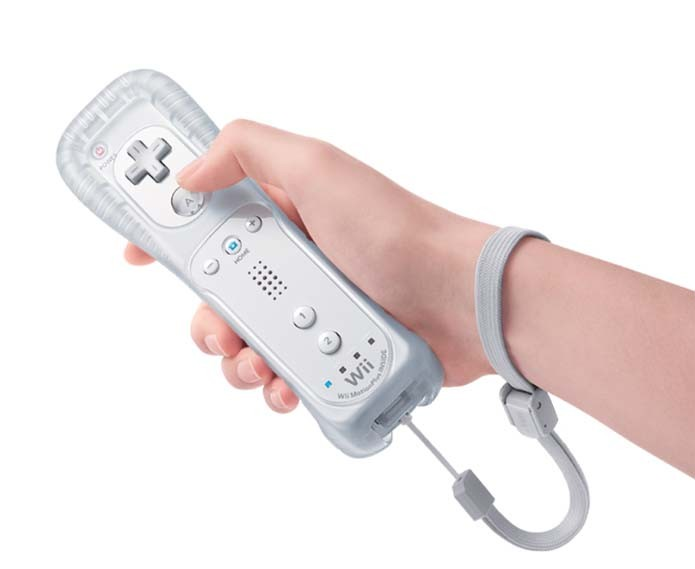
\includegraphics[scale=0.22]{wii}
\centering
\caption{Wii Remote (o Telecomando Wii)}
\label{fig:wii}
\end{figure}
\\Le strategie di marketing  del nuovo millennio puntano a far conoscere il mondo videoludico a quanta più gente possibile, anche alle fasce di età che non avevano mai dimostrato interesse per questo campo. La prima console che è riuscita in questa impresa è stata Nintendo Wii. La famosa console è riuscita a sbaragliare le rivali Play Station 3 e Xbox360, vendendo oltre cento milioni di copie. Il successo della Wii è dovuto al suo rivoluzionario metodo di motion detection, che è riuscito ad ottenere l’interesse di ogni fascia d’etá. Il Wii Remote (Figura~\ref{fig:wii}) rappresenta il concetto di un oggetto nel videogioco, per esempio una spada. Al movimento del telecomando, un sensore intercetta il movimento effettuato e lo invia al gioco, che reagisce di conseguenza. Lo straordinario numero di vendite è stato dettato proprio da questo banale concetto: la sensazione di immersione nel gioco che hanno i giocatori.\\L’avvicinamento di più pubblico nel mondo videoludico negli ultimi anni è stata purtroppo anche causa di una grave crisi.\\I videogiochi si sono dovuti adattare alle esigenze della maggioranza, maturando cambiamenti tra i quali:
\begin{itemize}
\item Abbassamento della difficoltà \\
Il videogioco è diventato molto più facile. La mentalità della maggior parte delle persone è fissa sul pensiero che vincere è gratificante e perdere è frustrante. Se il giocatore medio tende a vincere di più è quindi anche più invogliato a continuare il gioco.
\item Mire sulla grafica \\
L’aumento di prestazioni grafiche è stato possibile grazie all’evoluzione dell’hardware. Come natura umana impone, le persone sono molto più attratte da ciò che è piacevole alla vista rispetto al contrario.
\item Mire sui social \\
Al giorno d’oggi, Sony, Microsoft e Nintendo si stanno facendo guerra per creare Console sempre più social. Proprio come in un social network, i giocatori hanno l’esigenza di restare in contatto tra loro e mostrare come vivono la loro esperienza di gioco grazie al sistema di \gls{achievement}.
\item Mire sulla trama \\
Il giocatore medio è sempre più convinto che il videogioco non sia altro che un’esperienza cinematografica in cui lui stesso è il protagonista. Le azioni del protagonista possono modificare la storia in base alle scelte fatte in precedenza. Basta pensare al famoso titolo \textit{Beyond Two Souls} (Figura~\ref{fig:beyond}), il quale ha ben ventitre possibili finali diversi.
\begin{figure}[!ht]
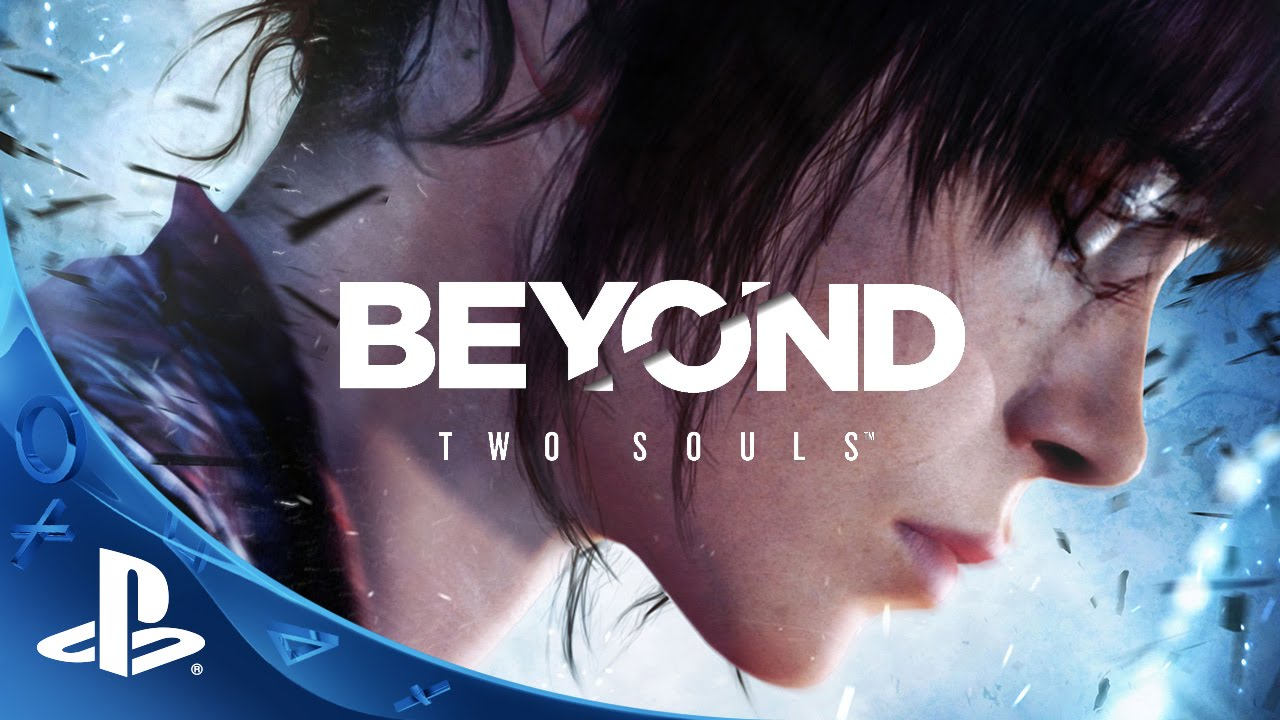
\includegraphics[scale=0.20]{beyond}
\centering
\caption{Beyond Two Souls (sviluppato da Quantic Dream)}
\label{fig:beyond}
\end{figure}
\item Gratuità \\
Sono sempre meno le persone disposte a comprare un videogioco per paura che l’acquisto non valga i soldi spesi. A questo proposito sono nati i \gls{f2p}, ovvero una categoria di videogiochi che offrono il loro intero contenuto gratuitamente. Ovviamente i produttori sono comunque costretti a cercare guadagno con altri metodi. Può avvenire grazie a strumenti come pubblicità e sponsor o tramite agevolazioni che il gioco può offrire al giocatore in cambio di soldi reali. Chiaramente è possibile giocare anche senza pagare, ma chi lo fa è agevolato rispetto a tutti gli altri utenti. Quest’ultimo metodo è particolarmente gettonato soprattutto nei giochi per smartphone.
\item Multiplayer Online \\
Ogni titolo di successo non può essere definito tale se non possiede il multiplayer. Alcuni giochi sono addirittura concepiti per funzionare solo ed esclusivamente online (come gli \gls{mmorpg}), e la maggior parte di questi richiede collaborazione tra i giocatori. Questo aspetto è stato favorito anche dalla nascita di mezzi di comunicazione come TeamSpeak o Discord. Ovviamente ci sono alcuni rari casi in cui qualche gioco è provvisto di sola modalità SinglePlayer ed è comunque un successo, ma può dipendere da molti altri fattori.
\item Notizie \\
È normale al giorno d’oggi imbattersi in recensioni di titoli, a volte addirittura prima ancora che questi ultimi escano. Quando ancora internet non esisteva, per acquistare un gioco ci si affidava principalmente alla copertina. Ora il web è addirittura colmo di guide che indicano passo dopo passo come terminare un videogioco al 100\%.
\item Diminuzione di hacking \\
Così come nelle competizioni sportive è vietato il doping degli atleti, nelle normali sessioni di gioco Online e soprattutto negli \gls{esport} è estremamente vietato l’hacking.
Con hacking o cheating si intende l’uso di software di terze parti mirati a modificare direttamente il codice di gioco per ottenere effetti benefici normalmente impossibili su uno o più partecipanti. Cheat famosi sono Aimbot (mira automatica in videogame \gls{fps}) e Wallhack (visione attraverso muri di altri giocatori o strumenti, sempre negli stessi generi di gioco). Per fortuna negli ultimi tempi gli hacker sono diminuiti, sia per principi morali sia grazie a sistemi di ban immediato come il VAC (Valve Anti-Cheat), inventato appunto dalla prestigiosissima azienda videoludica \textit{Valve}.
\end{itemize}
C’è da sottolineare che le nuove console non hanno più lo stesso ciclo vitale delle loro predecessori. Una console di nuova generazione ha tempi di vita molto brevi rispetto al passato perché non  sono diventate altro che dei veri e propri computer, con prestazioni più basse, prezzi più alti e limitazioni negli usi. Su alcune delle ultime console uscite in commercio è perfino possibile installare un sistema Linux. Addirittura, all’\gls{e3} di Giugno 2016 si è scoperto che Microsoft per mostrare i nuovi giochi di Xbox One ha usato delle postazioni con dei PC al posto delle console.\\La predisposizione ad acquistare un PC rispetto ad una console sta aumentando nel tempo.
